\documentclass[11pt,a4paper,french,twoside]{PMCours}
\usepackage{hyperref}
\usepackage{lastpage}
\frenchbsetup{StandardLists=true}

\begin{document}
\TitreISN{Classe de Terminale}{Année 2021--2022}
{Numérique et Sciences Informatiques}{Épreuve de Spécialité - Sujet 1 - 3h30}

\medskip
{\large Dès que ce sujet vous est remis, assurez-vous qu’il est complet.
\textbf{Ce sujet comporte \pageref{LastPage} pages.}

\medskip
Chaque candidat traitera trois exercices au choix parmi les cinq proposés, 
chaque exercice étant noté sur sept points.

\medskip
\textbf{Les exercices seront rendus sur des copies séparées.}

\medskip
L'usage de tout document, calculatrice, etc... est interdit.

\medskip
\textbf{Les élèves rendront de manière impérative brouillons et sujet en même temps que leur composition.}}

\newpage
\section*{Exercice 1}
\emph{Cet exercice porte sur les bases de données relationnelles et le langage SQL}

\medskip
Cet exercice utilise les mots du langage SQL parmi :
\begin{verbatim}
SELECT, FROM, WHERE, JOIN, ON, INSERT INTO, DELETE FROM, 
VALUES, ORDER BY, ASC, DESC, DISTINCT, AS,
LIMIT, LIKE, IN, AND, OR, NOT, MIN, MAX, COUNT, SUM,
<, >, <=, >=, =, !=
\end{verbatim} 

\medskip
On rappelle que :
\begin{itemize}
\item \code{DISTINCT} utilisé après \code{SELECT} supprime les doublons dans les résultats des requêtes.
\item \verb'ORDER BY' permet de classer les résultats d'une requête (par ordre croissant \code{ASC} ou décroissant \code{DESC}) et obéit à la syntaxe : 
\begin{verbatim}
SELECT Attributs FROM Table WHERE Condition ORDER BY Attribut_de_classement ASC (ou DESC)
\end{verbatim}
\item \code{COUNT} renvoie le nombre de lignes dans la réponse à une requête et obéit à la syntaxe :
\begin{verbatim}
SELECT COUNT(Attribut) FROM Table WHERE Condition
\end{verbatim}
\item \code{MIN}, \code{MAX}, \code{SUM} s'utilisent de manière similaire.
\end{itemize}

%On rappelle que \verb's LIKE m', où \verb's' est le nom d'un attribut de type chaîne de caractères et \verb'm' est un motif de chaîne de caractères (contenant le caractère \verb"'_'" qui remplace n'importe quel caractère ou bien le caractère \verb"'%'" qui remplace n'importe quelle chaîne de caractères), renvoie un booléen indiquant si \verb's' est compatible avec le motif \verb'm'. Par exemple, \verb'"Bonjour" LIKE "B_nj%"' renvoie \verb'true'.
\medskip
Les types SQL des attributs utilisés dans cet exercice sont : 
\begin{verbatim}
Int, Float, String, Time, Date, Boolean
\end{verbatim} 
Le format retenu pour le type \verb'Time' est JJ/MM/AAAA (sans guillemets) et 
le format retenu pour le type \verb'Date' est HH:MM (sans guillemets).

\medskip
Un ingénieur en informatique doit concevoir une base de données relationnelle pour gérer la gare ferroviaire d'Arras. Cette base de données sert pour l'affichage des informations  que les voyageurs peuvent consulter, ainsi qu'aux mécaniciens chargés des opérations de maintenance. Pour cela, il envisage quatre relations, dont des extraits sont précisés ci-après. Les attributs soulignés d'une relation désignent la clé primaire. Les attributs suivis du symbole \verb'#' désignent des clés étrangères.

\begin{itemize}
\item \verb'Compagnie' (Nom : String, \underline{Symbole} : String, CodePays : String)
\begin{center}
\begin{tabular}{|c|c|c|}\hline
Nom & Symbole & CodePays\\\hline
SNCF & SNCF & F\\\hline
Train Toto & TT & F\\\hline
QuickTrains & QKT & GB\\\hline
\end{tabular}
\end{center}
%\caption{Extrait de la relation \textbf{Compagnie}}
\item \verb'Train' (\underline{RefComp} \verb'#' : String, \underline{Matricule} : String, Modele : String, AutonomieKm : Float, \\VitesseMaxKmH : Float, NbDePassagers : Int)
\begin{center}
\begin{tabular}{|c|c|c|c|c|c|}\hline
RefComp & Matricule & Modele & AutonomieKm & VitesseMaxKmH & NbDePassagers\\\hline
SNCF & SNCF 1234 & Alstom A380 & 2500 & 180 & 550\\\hline
TT & TT 547 & Siemens 737 & 1500 & 174,8 & 350\\\hline
QKT & QKT 78549 & Alstom A350 & 1700,5 & 130,0 & 350\\\hline
\end{tabular}
\end{center}
%\caption{Extrait de la relation \textbf{Train}}
\newpage
\item \verb'Voyage'
\begin{center}
\begin{tabular}{|c|c|c|c|c|c|}\hline
Reference & Type & Date & Horaire & Lieu & Retard\\\hline
TT 547 & Départ & 14/07/2022 & 14:30 & Londres & false\\\hline
QKT 78549 & Arrivée & 12/06/2022 & 13:00 & Paris & true\\\hline
QKT 78549 & Départ & 16/08/2022 & 07:15 & Berlin & false\\\hline
\end{tabular}
\end{center}
%\caption{Extrait de la relation \textbf{Voyage}}
Le lieu d'un voyage de type 'Départ' désigne la gare de destination de ce voyage. Le lieu d'un voyage de type 'Arrivée' désigne la gare de provenance de ce voyage. 
\item \verb'Operation' (\underline{Reference} \verb'#' : String, \underline{Date} : String, Horaire : Time, HoraireFin : Time, Nature : String)
\begin{center}
\begin{tabular}{|c|c|c|c|c|}\hline
Reference & Date & HoraireDebut & HoraireFin & Nature\\\hline
QKT 78549 & 17/06/2022 & 10:15 & 15:00 & Visite mensuelle des moteurs\\\hline
SNCF 1234 & 17/06/2022 & 09:00 & 13:00 & Réparation bogie avant\\\hline
SNCF 1234 & 01/05/2022 & 08:00 & 17:00 & Visite annuelle générale\\\hline
\end{tabular}
\end{center}
%\caption{Extrait de la relation \textbf{Operation}}
\end{itemize}

\begin{enumerate}
\item Écrire le schéma relationnel de la table \verb'Voyage' (sans préciser de clé primaire), en indiquant les éventuelles clés étrangères.
\item Pourquoi l'attribut \verb'Reference' ne peut pas être utilisé comme clé primaire pour la relation \verb'Voyage' ? Proposer une clé primaire valide, avec le minimum d'attributs, sachant qu'un train peut faire plusieurs rotations par jour vers une même destination.
\item Avec cette base de données, un train peut-il avoir plusieurs opérations de maintenance le même jour ? Justifier.
\item Qu'affiche la requête SQL suivante :
\begin{verbatim}
SELECT Reference FROM Operation WHERE Date = 17/06/2022 AND HoraireFin >= 14:00
\end{verbatim} 
\item Écrire une requête SQL qui affiche la référence des voyages retardés le 28 Janvier 2022.
\item Écrire une requête SQL qui ajoute à la relation \verb'Train' l'Alstom A321, de matricule QKT 2468, dont la vitesse maximale est de 160 km/h, pouvant emporter 760 passagers sur une distance maximale de 1000 km.
\item Écrire une requête SQL qui affiche les horaires des trains qui sont en provenance de Strasbourg le vendredi 1er avril 2022.
\item Écrire une requête SQL qui affiche le nombre de compagnies françaises (le code pays de la France étant F).
\item Écrire une requête SQL qui donne le nombre maximal de passagers qu'un modèle de train puisse transporter.\\
Écrire alors une requête SQL qui affiche les modèles de train qui peuvent transporter le plus de passagers.
%\item Écrire une requête SQL qui affiche le matricule des trains qui ont une opération de maintenance prévue entre le 1er et le 10 mai 2022.
\item On exécute la requête SQL suivante :
\begin{verbatim}
DELETE FROM Train WHERE Matricule = "SNCF 1234"
\end{verbatim} 
mais un message d'erreur est renvoyé, indiquant que l'opération est impossible. Expliquer pourquoi, en analysant les extraits de la base de données fournis, puis écrivez les commandes SQL complémentaires, en plus de celle-ci, afin que la requête puisse être réalisée avec succès.
\item Écrire une requête SQL qui affiche, sans répétition, le nom des compagnies ferroviaires qui possèdent au moins un Alstom A380.
\item Pour des raisons logistiques, une opération de maintenance ne peut pas être programmée pour un train un jour où il effectue un voyage. Ecrire une requête SQL qui affiche les matricules des trains qui ne respecteraient pas cette règle, c'est à dire pour lesquels une opération de maintenance serait prévue un jour où ils doivent voyager. 
\item Écrire une requête SQL qui affiche la liste des couples nom de compagnie / matricule de train de cette compagnie, triée dans l'ordre alphabétique décroissant des noms de compagnie.
%\item Ecrivez une requête SQL qui affiche le nombre total de passagers que la compagnie ferroviaire SNCF peut transporter avec ses trains.
% \item Ecrivez une requête SQL qui affiche les références des voyages de trains qui font escale à la gare de NataSahId. Par convention, on suppose qu'un train fait une escale lorsqu'il arrive puis repart le même jour.
%\item Ecrivez une requête SQL qui affiche les matricules des trains français qui ont une visite annuelle générale prévue en janvier 2022.
\item Écrire une requête SQL qui affiche le modèle de tous les trains qui arrivent de Londres ou partent vers Londres.
\end{enumerate}

\newpage
\section*{Exercice 2}
\emph{Cet exercice porte sur les réseaux et l'architecture machine.}

\medskip


\subsection*{Partie 1 : Protocole RIP}
On considère le réseau suivant (chaque routeur est repéré par une lettre) :
\begin{center}
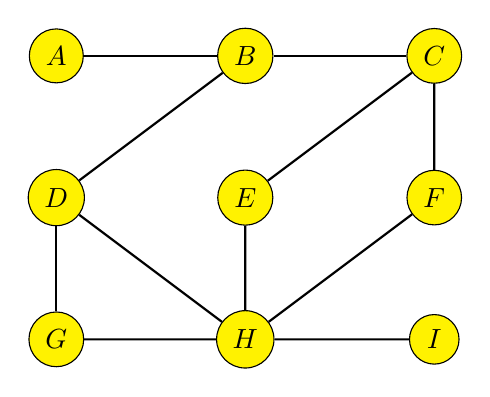
\begin{tikzpicture}[xscale=0.8,yscale=0.8]
% Styles (MODIFIABLES)
\tikzstyle{fleche}=[-,>=latex,thick]
\tikzstyle{noeud}=[fill=yellow,circle,draw]
\tikzstyle{feuille}=[fill=orange,circle,draw]
% Dimensions (MODIFIABLES)
\def\DistanceInterNiveaux{3}
\def\DistanceInterFeuilles{2}
% Dimensions calculées (NON MODIFIABLES)
\def\NiveauA{(-0)*\DistanceInterNiveaux}
\def\NiveauB{(-.75)*\DistanceInterNiveaux}
\def\NiveauC{(-1.5)*\DistanceInterNiveaux}
\def\InterFeuilles{(.75)*\DistanceInterFeuilles}
% Noeuds (MODIFIABLES : Styles et Coefficients d'InterFeuilles)
\node[noeud] (Ri) at ({(4)*\InterFeuilles},{\NiveauC}) {$I$};
\node[noeud] (Rh) at ({(2)*\InterFeuilles},{\NiveauC}) {$H$};
\node[noeud] (Rg) at ({(0)*\InterFeuilles},{\NiveauC}) {$G$};
\node[noeud] (Rf) at ({(4)*\InterFeuilles},{\NiveauB}) {$F$};
\node[noeud] (Re) at ({(2)*\InterFeuilles},{\NiveauB}) {$E$};
\node[noeud] (Rd) at ({(0)*\InterFeuilles},{\NiveauB}) {$D$};
\node[noeud] (Rc) at ({(4)*\InterFeuilles},{\NiveauA}) {$C$};
\node[noeud] (Rb) at ({(2)*\InterFeuilles},{\NiveauA}) {$B$};
\node[noeud] (Ra) at ({(0)*\InterFeuilles},{\NiveauA}) {$A$};
% Arcs (MODIFIABLES : Styles)
\draw[fleche] (Ra)--(Rb);
\draw[fleche] (Rb)--(Rc);
\draw[fleche] (Rb)--(Rd);
\draw[fleche] (Rc)--(Re);
\draw[fleche] (Rc)--(Rf);
\draw[fleche] (Rd)--(Rg);
%\draw[fleche,draw=white,double=black,very thick] (Re)--(Rf);
\draw[fleche] (Rd)--(Rh);
\draw[fleche] (Re)--(Rh);
\draw[fleche] (Rf)--(Rh);
\draw[fleche] (Rg)--(Rh);
\draw[fleche] (Rh)--(Ri);
\end{tikzpicture}
\end{center}
Pour les questions suivantes, on se place dans le cadre du protocole RIP.\\
Pour départager des chemins de même longueur, on considère qu'à chaque fois que cela était possible, les connexions ont été établies dans l'ordre alphabétique. \\
Ainsi, la liaison entre \code{A} et \code{B} a été créée avant celle entre \code{A} et \code{D},...\\
De plus, un chemin entre deux routeurs est remplacé par un autre chemin uniquement si le nouveau chemin est strictement plus court.

\begin{enumerate}
    \item Quel est le chemin de B vers I ?
    \item Quelle est la distance maximale entre deux routeurs de ce réseau ? 
    \item Recopier sur votre copie et compléter la table de routage du routeur H (sur le modèle de la table du {\bf 4)}:
    \begin{center}
        \begin{tabular}{|c|c|c|}\hline
            Destination&Routeur suivant&Distance\\ \hline
            $\vdots$ &$\vdots$&$\vdots$\\ \hline
            
        \end{tabular}
    \end{center}
    \item Une liaison directe a été ajoutée entre deux routeurs.
    La nouvelle table de routage du routeur G est alors :
    \begin{center}
        \begin{tabular}{|c|c|c|}\hline
            Destination&Routeur suivant&Distance\\ \hline
            A&D &2 \\ \hline 
            B&D &2 \\ \hline 
            C&D &3 \\ \hline 
            D&D &1 \\ \hline 
            E&H &2 \\ \hline 
            F&H &2 \\ \hline  
            H&H &1 \\ \hline
            I&H &2 \\ \hline
 \end{tabular}
    \end{center}
    Entre quels routeurs la liaison a-t-elle été ajoutée ? Justifier brièvement.
\end{enumerate}

\newpage
\subsection*{Partie 2 : Protocole OSPF}
On considère le réseau suivant (chaque routeur est repéré par une lettre) :
\begin{multicols}{2}
\begin{center}
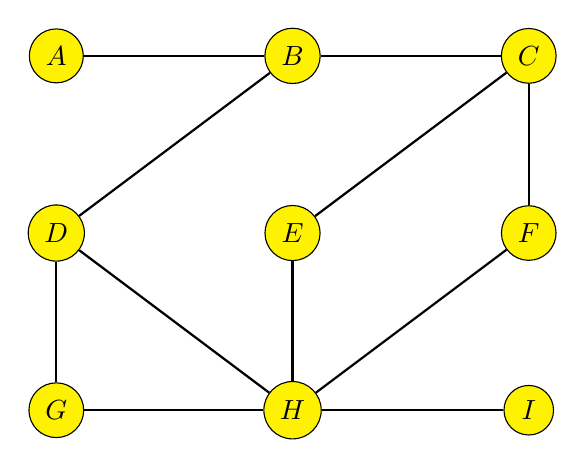
\begin{tikzpicture}[xscale=1,yscale=1]
% Styles (MODIFIABLES)
\tikzstyle{fleche}=[-,>=latex,thick]
\tikzstyle{noeud}=[fill=yellow,circle,draw]
\tikzstyle{feuille}=[fill=orange,circle,draw]
% Dimensions (MODIFIABLES)
\def\DistanceInterNiveaux{3}
\def\DistanceInterFeuilles{2}
% Dimensions calculées (NON MODIFIABLES)
\def\NiveauA{(-0)*\DistanceInterNiveaux}
\def\NiveauB{(-.75)*\DistanceInterNiveaux}
\def\NiveauC{(-1.5)*\DistanceInterNiveaux}
\def\InterFeuilles{(.75)*\DistanceInterFeuilles}
% Noeuds (MODIFIABLES : Styles et Coefficients d'InterFeuilles)
\node[noeud] (Ri) at ({(4)*\InterFeuilles},{\NiveauC}) {$I$};
\node[noeud] (Rh) at ({(2)*\InterFeuilles},{\NiveauC}) {$H$};
\node[noeud] (Rg) at ({(0)*\InterFeuilles},{\NiveauC}) {$G$};
\node[noeud] (Rf) at ({(4)*\InterFeuilles},{\NiveauB}) {$F$};
\node[noeud] (Re) at ({(2)*\InterFeuilles},{\NiveauB}) {$E$};
\node[noeud] (Rd) at ({(0)*\InterFeuilles},{\NiveauB}) {$D$};
\node[noeud] (Rc) at ({(4)*\InterFeuilles},{\NiveauA}) {$C$};
\node[noeud] (Rb) at ({(2)*\InterFeuilles},{\NiveauA}) {$B$};
\node[noeud] (Ra) at ({(0)*\InterFeuilles},{\NiveauA}) {$A$};
% Arcs (MODIFIABLES : Styles)
\draw[fleche] (Ra)--(Rb);
\draw[fleche] (Rb)--(Rc);
\draw[fleche] (Rb)--(Rd);
\draw[fleche] (Rc)--(Re);
\draw[fleche] (Rc)--(Rf);
\draw[fleche] (Rd)--(Rg);
%\draw[fleche,draw=white,double=black,very thick] (Re)--(Rf);
\draw[fleche] (Rd)--(Rh);
\draw[fleche] (Re)--(Rh);
\draw[fleche] (Rf)--(Rh);
\draw[fleche] (Rg)--(Rh);
\draw[fleche] (Rh)--(Ri);
\end{tikzpicture}
\end{center}

\begin{tabular}{|l|l|l|}\hline
    Liaison& Type   & Débit\\\hline
    A$\leftrightarrow$B&Wi-Fi&20 Mbit/s \\\hline
    B$\leftrightarrow$C&Ethernet&20 Mbit/s \\\hline
    B$\leftrightarrow$D&Fast Ethernet&100 Mbit/s \\\hline
    C$\leftrightarrow$E&Fast Ethernet&100 Mbit/s \\\hline
    C$\leftrightarrow$F&Fast Ethernet&100 Mbit/s \\\hline
    D$\leftrightarrow$G&Fast Ethernet&100 Mbit/s  \\\hline
    D$\leftrightarrow$H&Ethernet&10 Mbit/s \\\hline
    E$\leftrightarrow$H&Fibre&1 Gbit/s \\\hline
    F$\leftrightarrow$H&Fast Ethernet&100 Mbit/s \\\hline
    G$\leftrightarrow$H&Ethernet&20 Mbit/s \\\hline
    H$\leftrightarrow$I&Fibre&1 Gbit/s \\\hline
 \end{tabular}
\end{multicols}
Pour les questions suivantes, on se place dans le cadre du protocole OSPF.
On rappelle que pour ce protocole, le coût d'une liaison est 
$\text{coût}=\frac{10^8}{d}$ où $d$ est la bande passante en $bit/s$.
\begin{enumerate}
    \item Quel est le coût des liaisons GH et HI ? Détailler les calculs.
    \item Sans autres justifications, recopier sur votre copie le graphe et donner la pondération de chacun des arcs. 
    \item Quel est le coût total du chemin B-D-H-I ?
    \item En justifiant brièvement, quel est le chemin le moins coûteux allant de B à I ?
\end{enumerate}

\subsection*{Partie 3 : Architecture}
On s'intéresse maintenant à une station météo gérée par un Raspberry~Pi. 

Voici le schéma général du Raspberry~Pi :
\begin{center}
    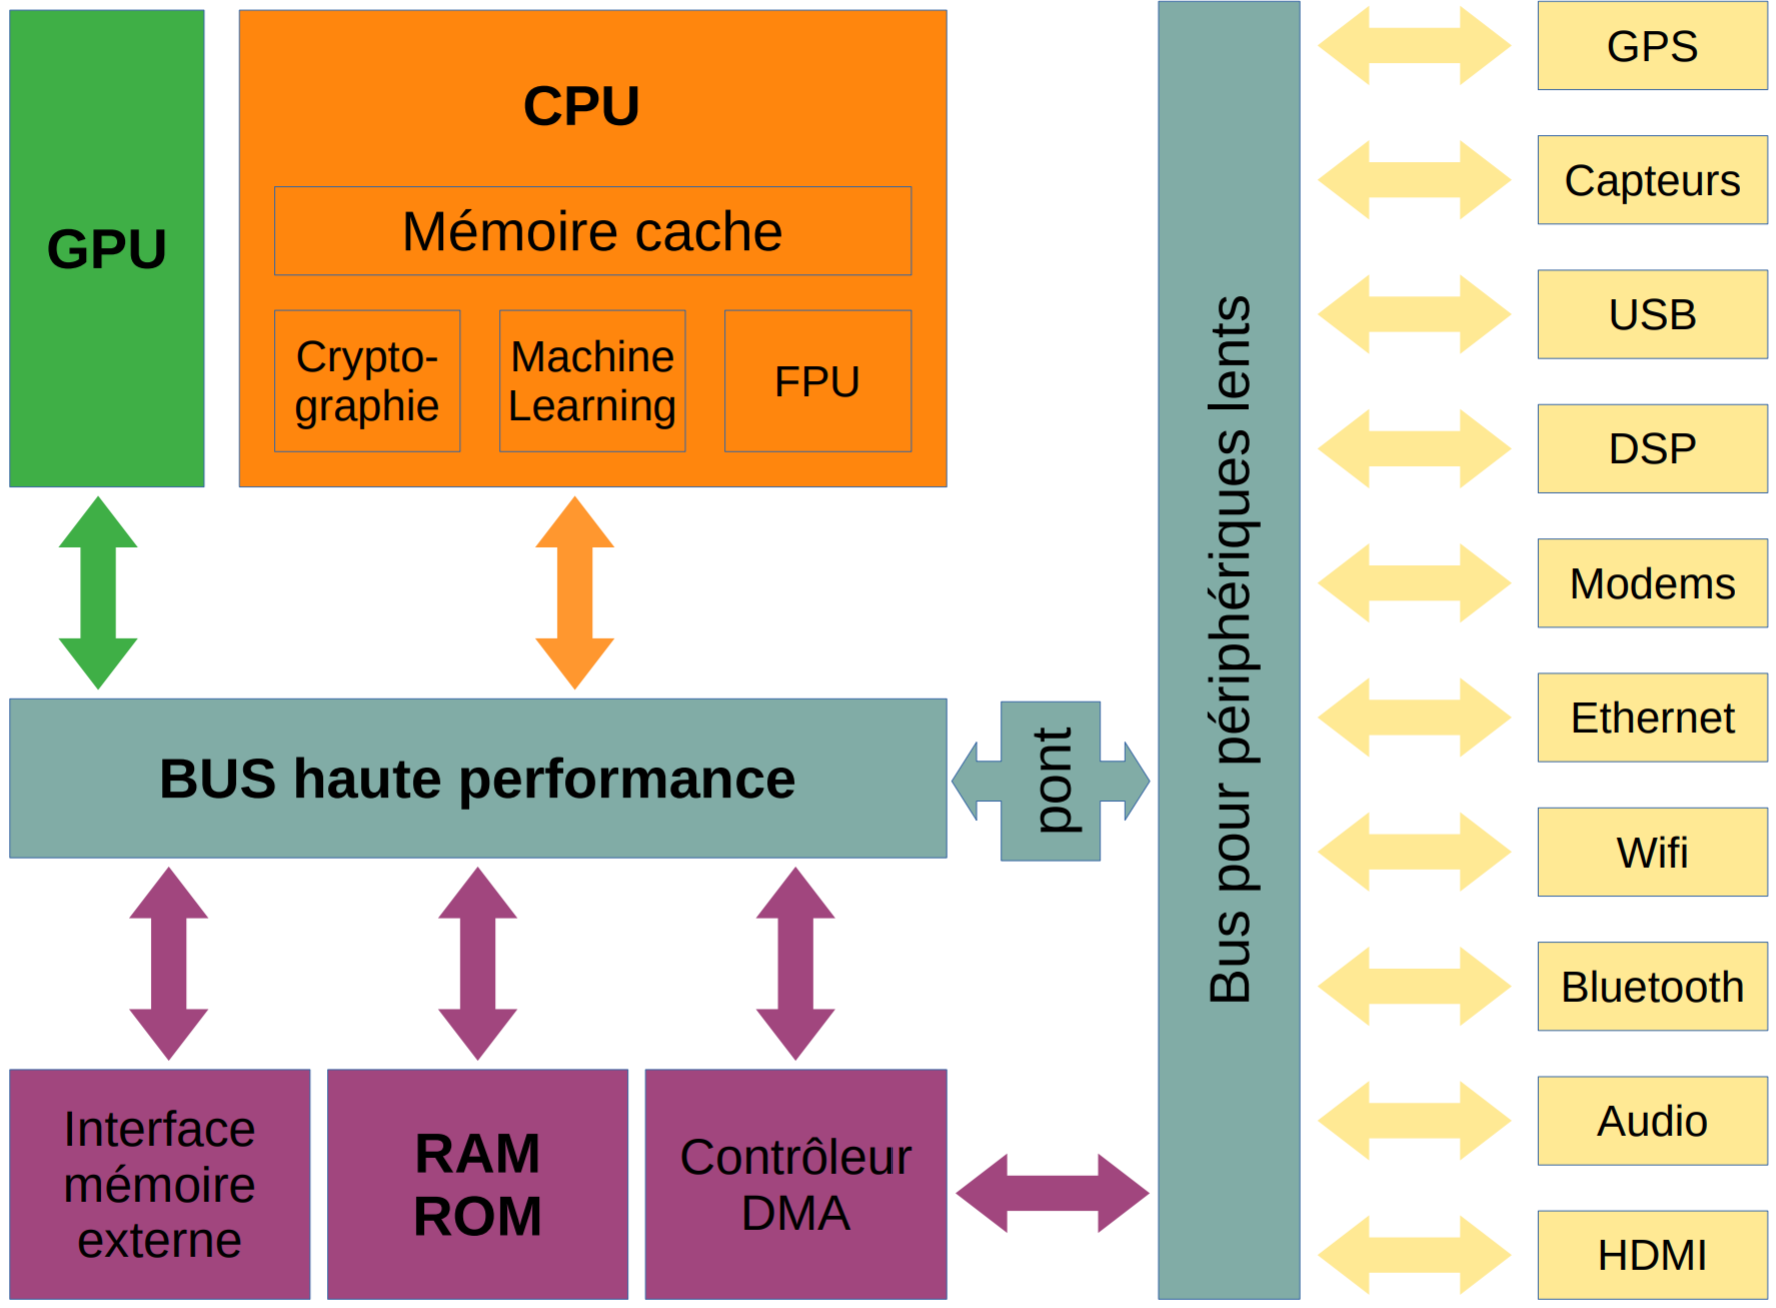
\includegraphics[width=10cm]{SchemaSoc.png}
\end{center}

Ce Raspberry~Pi est connecté au réseau internet via une liaison wifi. Il est 
relié directement avec la plupart de ses capteurs, sauf l'anémomètre à qui il 
est connecté par Bluetooth. Il dispose d'un stockage persistant grâce à un
disque SSD externe USB. Il n'a pas d'écran.  

\begin{enumerate}
    \item Donner la liste des modules d'entrée sortie (à droite dans le schéma) 
    nécessaires au bon fonctionnement de la station météo.
    \item Les processus s'exécutant sur le Raspberry~Pi ne doivent surtout pas
    s'arrêter. Expliquer ce qu'on appelle un interblocage.
\end{enumerate}

\newpage
\section*{Exercice 3}
\emph{Cet exercice porte sur l'algorithmique et la programmation en Python. Il aborde les notions
de tableaux de tableaux et d'algorithmes de parcours de tableaux.}

\subsection*{Partie A : Représentation d'un labyrinthe}
On modélise un labyrinthe par un tableau à deux dimensions à $n$ lignes et $m$ colonnes avec $n$ et
$m$ des entiers strictement positifs.

Les lignes sont numérotées de $0$ à $n-1$ et les colonnes de $0$ à $m-1$.
La case en haut à gauche est repérée par $(0,0)$ et la case en bas à droite par $(n-1,m-1)$.

Dans ce tableau :
\begin{itemize}
\item 0 représente une case vide, hors case de départ et arrivée,
\item 1 représente un mur,
\item 2 représente le départ du labyrinthe,
\item 3 représente l'arrivée du labyrinthe.
\end{itemize}
Ainsi, en Python, le labyrinthe ci-dessous est représentée par le tableau de tableaux \code{lab1}.

\begin{multicols}{2}
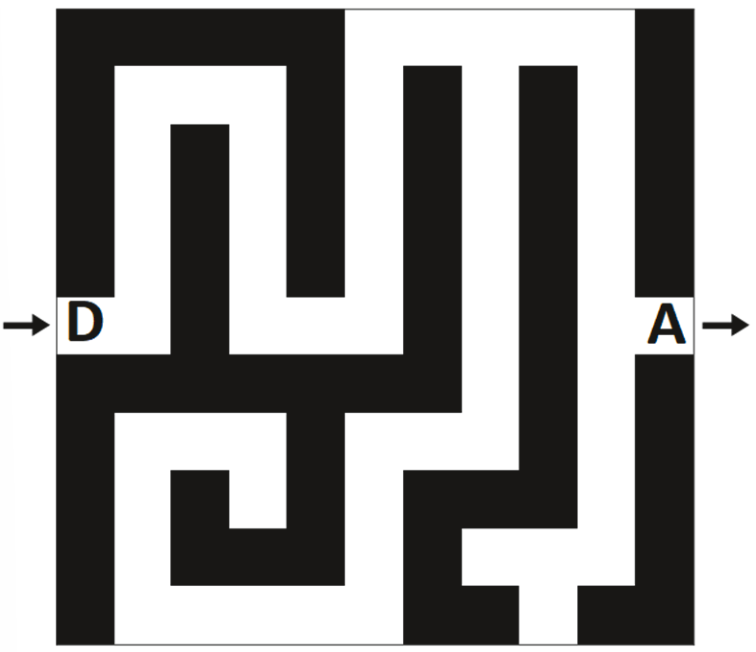
\includegraphics[width=6cm]{BacBlanc2Sujet1_NSI2122-img1.png}

\begin{alltt}
lab1 = [[1, 1, 1, 1, 1, 0, 0, 0, 0, 0, 1],
        [1, 0, 0, 0, 1, 0, 1, 0, 1, 0, 1],
        [1, 0, 1, 0, 1, 0, 1, 0, 1, 0, 1],
        [1, 0, 1, 0, 1, 0, 1, 0, 1, 0, 1],
        [1, 0, 1, 0, 1, 0, 1, 0, 1, 0, 1],
        [2, 0, 1, 0, 0, 0, 1, 0, 1, 0, 3],
        [1, 1, 1, 1, 1, 1, 1, 0, 1, 0, 1],
        [1, 0, 0, 0, 1, 0, 0, 0, 1, 0, 1],
        [1, 0, 1, 0, 1, 0, 1, 1, 1, 0, 1],
        [1, 0, 1, 1, 1, 0, 1, 0, 0, 0, 1],
        [1, 0, 0, 0, 0, 0, 1, 1, 0, 1, 1]]
\end{alltt}
\end{multicols}

\begin{enumerate}
\item Le labyrinthe ci-dessous est censé être représenté par le tableau de tableaux \code{lab2}.
Cependant, dans ce tableau, un mur se trouve à la place du départ du labyrinthe.
Donner une instruction permettant de placer le départ au bon endroit dans \code{lab2}.
\begin{multicols}{2}
    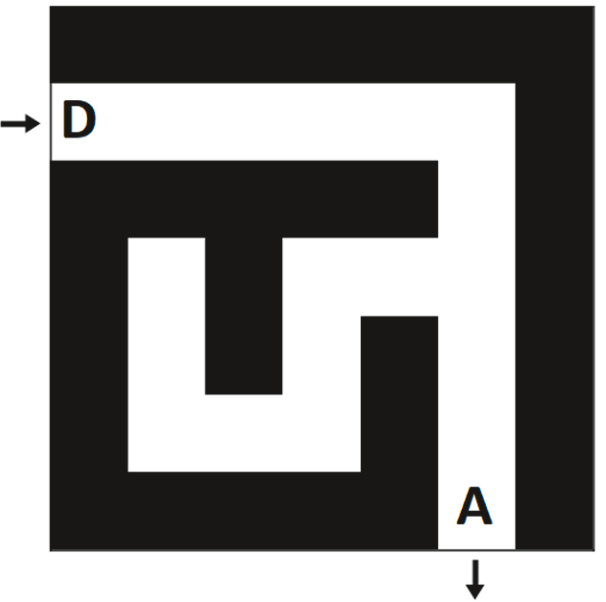
\includegraphics[width=4cm]{BacBlanc2Sujet1_NSI2122-img2.png}

\begin{alltt}
lab2 = [[1, 1, 1, 1, 1, 1, 1],
        [1, 0, 0, 0, 0, 0, 1],
        [1, 1, 1, 1, 1, 0, 1],
        [1, 0, 1, 0, 0, 0, 1],
        [1, 0, 1, 0, 1, 0, 1],
        [1, 0, 0, 0, 1, 0, 1],
        [1, 1, 1, 1, 1, 3, 1]]
\end{alltt}
\end{multicols}
\item Écrire une fonction \code{est\_valide(i, j, n, m)} qui renvoie \code{True} si le couple $(i,j)$
correspond à des coordonnées valides pour un labyrinthe de taille $(n,m)$, et \code{False} sinon.

On donne ci-dessous des exemples d'appels.
\begin{alltt}
>>> est\_valide(5, 2, 10, 7)
True
>>> est\_valide(10, 4, 10, 7)
False
\end{alltt}
\item On suppose que le départ d'un labyrinthe est toujours indiqué, mais on ne fait aucune
supposition sur son emplacement. Recopier et compléter les lignes incomplètes de la fonction \code{depart(lab)} ci-dessous de sorte qu'elle renvoie, sous la forme d'un tuple, les coordonnées du départ d'un labyrinthe (représenté par le paramètre \code{lab}). 

Par exemple, l'appel \code{depart(lab1)} doit renvoyer le tuple \code{(5, 0)}.
\begin{Python}
def depart(lab) :
    n = len(lab)
    m = len(lab[0])
    for i in #àcompléter1 : 
    	for j in #àcompléter2 :
    		if lab[i][j] #àcompléter3 :
    			return (i,j)
\end{Python}
\item Écrire une fonction \code{nb\_cases\_vides(lab)} qui renvoie le nombre de cases vides d'un
labyrinthe (comprenant donc l'arrivée et le départ).

Par exemple, l'appel \code{nb\_cases\_vides(lab2)} doit renvoyer la valeur \code{19}.
\end{enumerate}

\subsection*{Partie B : Recherche d'une solution dans un labyrinthe}
On suppose dans cette partie que les labyrinthes possèdent un unique chemin allant du départ
à l'arrivée sans repasser par la même case. Dans la suite, c'est ce chemin que l'on appellera
solution du labyrinthe.

Pour déterminer la solution d'un labyrinthe, on parcourt les cases vides de proche en proche.
Lors d'un tel parcours, afin d'éviter de tourner en rond, on choisit de marquer les cases visitées.
Pour cela, on remplace la valeur d'une case visitée dans le tableau représentant le labyrinthe
par la valeur $4$.
\begin{enumerate}
\item On dit que deux cases d'un labyrinthe sont voisines si elles ont un côté commun.
On considère une fonction \code{voisines(i, j, lab)} qui prend en arguments deux entiers $i$
et $j$ représentant les coordonnées d'une case et un tableau \code{lab} qui représente un labyrinthe.

Cette fonction renvoie la liste des coordonnées des cases voisines de la case de
coordonnées $(i,j)$ qui sont valides, non visitées et qui ne sont pas des murs. L'ordre des
éléments de cette liste n'importe pas.

Ainsi, l'appel \code{voisines(1, 1, [[1, 1, 1], [4, 0, 0], [1, 0, 1]])} renvoie la
liste \code{[(2, 1), (1, 2)]}.

Que renvoie l'appel \code{voisines(1, 2, [[1, 1, 4], [0, 0, 0], [1, 1, 0]])} ?
\item On souhaite stocker la solution dans une liste \code{chemin}. Cette liste contiendra les
coordonnées des cases de la solution, dans l'ordre. Pour cela, on procède de la façon
suivante.
\begin{itemize}
\item Initialement :
\begin{itemize}
\item déterminer les coordonnées du départ : c'est la première case à visiter ;
\item ajouter les coordonnées de la case départ à la liste \code{chemin}.
\end{itemize}
\item Tant que l'arrivée n'a pas été atteinte :
\begin{itemize}
\item on marque la case visitée avec la valeur 4 ;
\item si la case visitée possède une case voisine libre, la première case de la liste
renvoyée par la fonction \code{voisines} devient la prochaine case à visiter et on
ajoute à la liste \code{chemin} ;
\item sinon, il s'agit d'une impasse. On supprime alors la dernière case dans la liste
\code{chemin}. La prochaine case à visiter est celle qui est désormais en dernière
position de la liste \code{chemin}.
\end{itemize}
\end{itemize}

\begin{enumerate}
\item Le tableau de tableaux \code{lab3} ci-dessous représente un labyrinthe.
\begin{alltt}
lab3 = [[1, 1, 1, 1, 1, 1],
        [2, 0, 0, 0, 0, 3],
        [1, 0, 1, 0, 1, 1],
        [1, 1, 1, 0, 0, 1]]
\end{alltt}
La suite d'instructions ci-dessous simule le début des modifications subies par la liste
\code{chemin} lorsque l'on applique la méthode présentée.
\begin{alltt}
# entrée: (1, 0), sortie (1, 5)
chemin = [(1, 0)]
chemin.append((1, 1))
chemin.append((2, 1))
chemin.pop()
chemin.append((1, 2))
chemin.append((1, 3))
chemin.append((2, 3))
\end{alltt}
Compléter cette suite d'instructions jusqu'à ce que la liste \code{chemin} représente la
solution. \emph{Rappel : la méthode \code{pop} supprime le dernier élément d'une liste et renvoie cet
élément.}
\item Recopier et compléter la fonction \code{solution(lab)} donnée ci-dessous de sorte qu'elle
renvoie le chemin solution du labyrinthe représenté par le paramètre \code{lab}.
On pourra pour cela utiliser la fonction \code{voisines}.
\begin{alltt}
def solution(lab):
    chemin = [depart(lab)]
    case = chemin[0]
    i = case[0]
    j = case[1]
    ...
\end{alltt}
Par exemple, l'appel \code{solution(lab2)} doit renvoyer \code{[(1, 0), (1, 1), (1, 2),
(1, 3), (1, 4), (1, 5), (2, 5), (3, 5), (4, 5), (5, 5), (6, 5)]}.
\end{enumerate}
\end{enumerate}


\newpage
\section*{Exercice 4}
\emph{Cet exercice porte sur les arbres, les dictionnaires et la programmation orientée objet.}

\medskip
Une agence immobilière développe un programme pour gérer les biens immobiliers qu'elle
propose à la vente.

Dans ce programme, pour modéliser les données de biens immobiliers, on définit une classe
\code{Bim} avec les attributs suivants :
\begin{itemize}
\item \code{nt} de type \code{str} représente la nature du bien (appartement, maison, bureau,
commerces, … ) ;
\item \code{sf} de type \code{float} est la surface du bien ;
\item \code{pm} de type \code{float} est le prix moyen par m² du bien qui dépend de son
emplacement.
\end{itemize}

La classe \code{Bim} possède une méthode \code{estim\_prix} qui renvoie une estimation du prix du
bien. Le code (incomplet) de la classe \code{Bim} est donné ci-dessous :
\begin{Python*}
class Bim:
    def __init__(self, nature, surface, prix_moy):
        ...
    def estim_prix(self):
        return self.sf * self.pm
\end{Python*}

\begin{enumerate}
\item Recopier et compléter le code du constructeur de la classe \code{Bim}.
\item On exécute l'instruction suivante :

\medskip
\code{b1 = Bim('maison', 70.0, 2000.0)}

Que renvoie l'instruction \code{b1.estim\_prix()} ? Préciser le type de la valeur renvoyée.
\item On souhaite affiner l'estimation du prix d'un bien en prenant en compte sa nature :
\begin{itemize}
\item pour un bien dont l'attribut \code{nt} est \code{'maison'} la nouvelle estimation du prix est le
produit de sa surface par le prix moyen par m² multiplié par $1,\!1$ ;
\item pour un bien dont l'attribut \code{nt} est \code{'bureau'} la nouvelle estimation du prix est le
produit de sa surface par le prix moyen par m² multiplié par $0,\!8$ ;
\item pour les biens d'autres natures, l'estimation du prix ne change pas.
\end{itemize}
Modifier le code de la méthode \code{estim\_prix} afin de prendre en compte ce changement
de calcul.
\item 
\begin{enumerate} 
\item Recopier et compléter le code Python ci-dessous afin d'obtenir une fonction \code{nb\_maison} qui prend en argument une liste Python de biens immobiliers de type \code{Bim} et qui renvoie le nombre d'objets de nature \code{'maison'} contenus dans la liste \code{lst}.
\begin{Python}
def nb_maison(lst) : 
	#à compléter1
	for bien in lst : 
		if #à compléter2 :
			c=c+1
	return c
\end{Python}
On veut maintenant utiliser une structure de dictionnaire pour compter le nombre de biens de chaque type immobilier.
\item On crée la variable \code{dict=\{'AB' : 3, 'CD' : 4\}}.\\
Pour chacune des commandes suivantes, en précisant votre réponse, dire si il y a une valeur renvoyée, une modification apportée à \code{dict} ou une erreur : 
\begin{itemize} 
\item \code{dict['CD']=8}
\item \code{dict('AB')}
\item \code{dict['AB']}
\item \code{dict['AB']+=1}
\item \code{dict['EF']=1}
\item \code{'AB' in dict}
\item \code{'XY' in dict}
\end{itemize} 
\item Écrire le code d'une fonction \code{nb\_type} qui prend en argument une liste Python de biens immobiliers de type \code{Bim} et qui renvoie un dictionnaire comptabilisant le nombre de biens de chaque type contenus dans la liste \code{lst}.\\
Par exemple, la fonction renverra \code{\{'maison' : 3, 'appartement' : 7, 'garage' : 2\}} si il y a 3 maisons, 7 appartements et 2 garages dans la liste.
\end{enumerate}    
\item Pour une recherche efficace des biens immobiliers selon le critère de leur surface, on
stocke les objets de type \code{Bim} dans un arbre binaire de recherche, nommé \code{abr}. Pour tout
nœud de cet arbre :
\begin{itemize}
\item tous les objets de son sous-arbre gauche ont une surface inférieure ou égale à la
surface de l'objet contenue dans ce nœud ;
\item tous les objets de son sous-arbre droit ont une surface strictement supérieure à la
surface de l'objet contenue dans ce nœud.
\end{itemize}

L'objet \code{abr} dispose des méthodes suivantes :
\begin{itemize}
\item[] \code{abr.est\_vide()} : renvoie \code{True} si \code{abr} est vide et \code{False} sinon.
\item[] \code{abr.get\_v()} : renvoie l'élément (de type \code{Bim}) situé à la racine de \code{abr} si \code{abr} n'est
pas vide et \code{None} sinon.
\item[] \code{abr.get\_g()} : renvoie le sous-arbre gauche de \code{abr} si \code{abr} n'est pas vide et \code{None}
sinon.
\item[] \code{abr.get\_d()} : renvoie le sous-arbre droit de \code{abr} si \code{abr} n'est pas vide et \code{None} sinon.
\end{itemize}

\begin{enumerate}
\item Dans cette question, on suppose que l'arbre binaire \code{abr} a la forme ci-dessous :
\begin{center}
   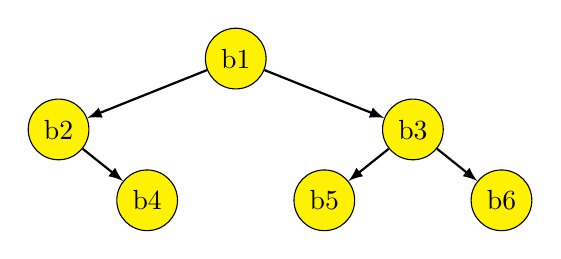
\begin{tikzpicture}[xscale=.5,yscale=.4]
% Styles (MODIFIABLES)
\tikzstyle{fleche}=[->,>=latex,thick]
\tikzstyle{noeud}=[fill=yellow,circle,draw]
\tikzstyle{feuille}=[fill=orange,circle,draw]
% Dimensions (MODIFIABLES)
\def\DistanceInterNiveaux{3}
\def\DistanceInterFeuilles{2}
% Dimensions calculées (NON MODIFIABLES)
\def\NiveauA{(-0)*\DistanceInterNiveaux}
\def\NiveauB{(-.75)*\DistanceInterNiveaux}
\def\NiveauC{(-1.5)*\DistanceInterNiveaux}
\def\NiveauD{(-2.25)*\DistanceInterNiveaux}
\def\InterFeuilles{(.75)*\DistanceInterFeuilles}
% Noeuds (MODIFIABLES : Styles et Coefficients d'InterFeuilles)
\node[noeud] (R) at ({(0)*\InterFeuilles},{\NiveauA}) {b1};
\node[noeud] (Ra) at ({(-3)*\InterFeuilles},{\NiveauB}) {b2};
\node[noeud] (Rb) at ({(3)*\InterFeuilles},{\NiveauB}) {b3};
\node[noeud] (Rab) at ({(-1.5)*\InterFeuilles},{\NiveauC}) {b4};
\node[noeud] (Rba) at ({(1.5)*\InterFeuilles},{\NiveauC}) {b5};
\node[noeud] (Rbb) at ({(4.5)*\InterFeuilles},{\NiveauC}) {b6};
% Arcs (MODIFIABLES : Styles)
\draw[fleche] (R)--(Ra);
\draw[fleche] (R)--(Rb);
\draw[fleche] (Ra)--(Rab);
\draw[fleche] (Rb)--(Rba);
\draw[fleche] (Rb)--(Rbb);
\end{tikzpicture}
\end{center}
Donner la liste les biens \code{b1}, \code{b2}, \code{b3}, \code{b4}, \code{b5}, \code{b6} triée dans l'ordre croissant de leur surface.
\item Recopier et compléter le code de la fonction récursive \code{contient} donnée ci-dessous, qui
prend en arguments un nombre \code{surface} de type \code{float} et un arbre binaire de recherche
\code{abr} contenant des éléments de type \code{Bim} ordonnés selon leur attribut de surface \code{sf}. 

La fonction \code{contient(surface, abr)} renvoie \code{True} s'il existe un bien dans \code{abr} d'une surface supérieure ou égale à \code{surface} et \code{False} sinon.
\begin{Python*}
def contient(surface, abr):
    if abr.est_vide():
        return False
    elif abr.get_v().sf >= ……… :
        return True 
    else:
        return contient( surface , ……… ) 
\end{Python*}
\end{enumerate}
\end{enumerate}

\newpage
\section*{Exercice 5}
\emph{Notion abordée : structures de données : les piles.}

\medskip
Dans cet exercice, on considère une pile d'entiers positifs. On suppose que les quatre
fonctions suivantes ont été programmées préalablement en langage Python :
\begin{itemize}
\item[] \code{empiler(P, e)} : ajoute l'élément \code{e} sur la pile \code{P} ;
\item[] \code{depiler(P)} : enlève le sommet de la pile \code{P} et retourne la valeur de ce sommet ;
\item[] \code{est\_vide(P)} : renvoie \code{True} si la pile est vide et \code{False} sinon ;
\item[] \code{creer\_pile()} : renvoie une pile vide.
\end{itemize} 

\textbf{Dans cet exercice, seule l'utilisation de ces quatre fonctions sur la structure de
données pile est autorisée.}

\begin{enumerate} 
    \item Recopier le schéma ci-dessous et le compléter sur votre copie en exécutant
    les appels de fonctions donnés. On écrira ce que renvoie la fonction utilisée
    dans chaque cas, et on indiquera None si la fonction ne retourne aucune
    valeur.
    \begin{center}
        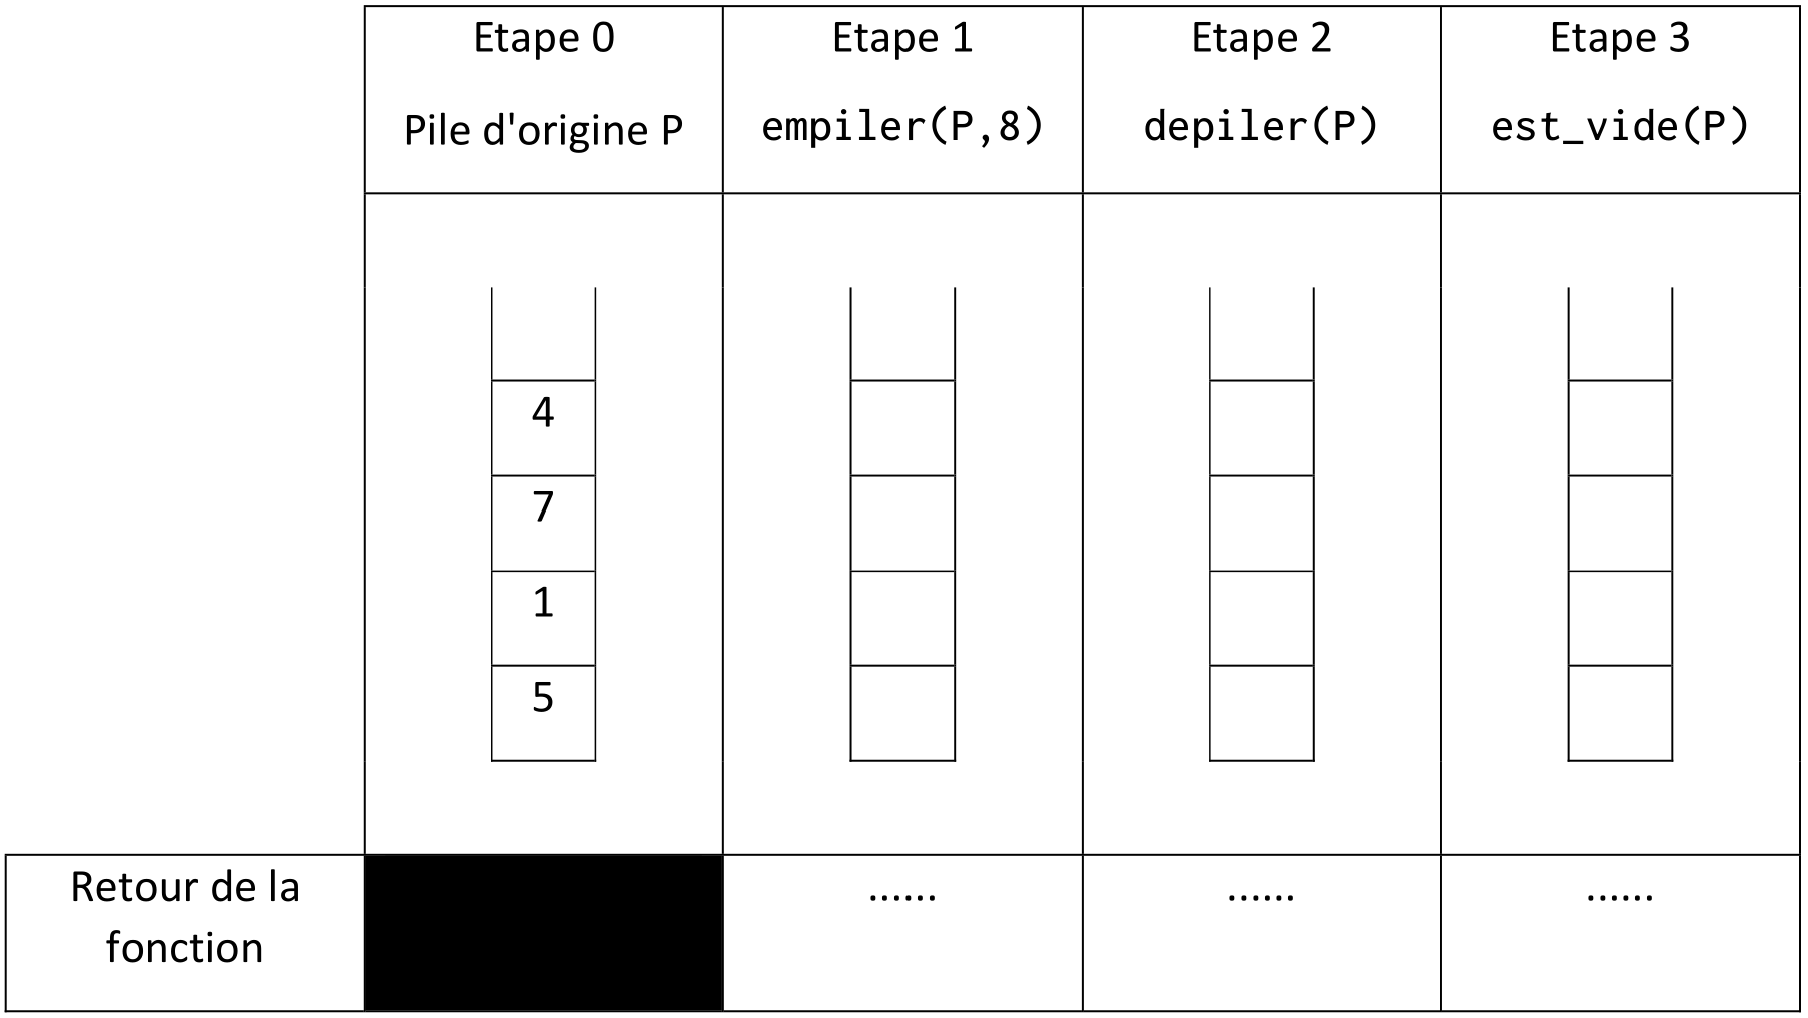
\includegraphics[width=0.8\linewidth]{BacBlanc2Sujet1_NSI2122-img3.png}
    \end{center}
    \item \begin{enumerate}
    \item On donne la fonction ci-dessous, qui prend en argument une pile \code{P} et renvoie
    un pile \code{Q} :
    \begin{Python}
    def transforme(P) :
        Q = creer_pile()
        while not est_vide(P) :
            v = depile(P)
            empile(Q,v)
        return (Q)
    \end{Python}
Si \code{P} est la pile à l'étape 0 de la {\bf question 1}, donner en justifiant la valeur de \code{P} et de \code{Q} après l'exécution de l'appel \code{transforme(P)} . 
    \item En s'inspirant du code de \code{transforme}, écrire le code d'une fonction \code{transforme2} qui prend comme argument une pile \code{P} et renvoie une pile \code{Q} comme ci-dessus mais cette fois en laissant \code{P} inchangée.\medskip\\
On signale que si \code{P} est une pile, alors la commande \code{R=P} crée un ''clone'' de \code{P} et que toute modification apportée à \code{P} se répercute sur \code{R} et vice-versa.
 \end{enumerate}    
    \item On souhaite connaître le nombre d'éléments d'une pile à l'aide d'une fonction \code{taille} telle qu'à la fin de l'exécution de cette fonction, la pile de départ soit inchangée.\\
Ainsi, si \code{P} est la pile à l'étape 0 de la {\bf question 1}, \code{taille(P)} renverra la valeur 4 et laissera \code{P} inchangée.
   
\begin{enumerate}
    \item Proposer une stratégie écrite en langage naturel et/ou expliquée à l'aide de
    schémas, qui permette de mettre en place une telle fonction.
    \item Donner le code Python de cette fonction \code{taille}. On pourra éventuellement utiliser des fonctions précédemment programmées.
\end{enumerate}

    \item \begin{enumerate}
    \item Recopier le code de la fonction suivante afin d'en faire une fonction prenant en entrée une liste Python \code{L} de types numériques et renvoyant le maximum de cette liste et l'indice où il a été rencontré.
\begin{Python}
def max_liste(L) : 
	max=#àcompléter1
	imax=#àcompléter2
	for k in #àcompléter3 :
		if L[k]>max : 
			#àcompléter4
			#àcompléter5
	return max,imax
\end{Python}
    \item Écrire en langage Python une fonction \code{maximum} recevant une pile \code{P} comme argument et qui renvoie la valeur maximale de cette pile et la position dans la pile de cet élément (\code{1} pour le sommet de la pile, \code{2} pour l'élément suivant,...) . \\
    On souhaite de plus que cette fonction laisse son argument \code{P} inchangé.\\
Ainsi, si \code{P} est la pile à l'étape 0 de la {\bf question 1}, \code{maximum(P)} renverra le tuple \code{7,2} et laissera \code{P} inchangée. \\   
On pourra éventuellement utiliser des fonctions précédemment programmées.
\end{enumerate}
\end{enumerate}
    
    
\end{document}
    
    